\documentclass[11 pt]{scrartcl}
\usepackage[header, margin, koma, stylish]{chen}
\usepackage{csquotes}
\usepackage{caption}
\usepackage{todonotes}

\pagestyle{fancy}
\fancyhf{}
\fancyhead[l]{CS 161 Notes}
\fancyhead[r]{Chufan Chen}
\cfoot{\thepage}

\newcommand{\tx}{\tilde{x}}
\newcommand{\eq}{\text{eq}}
\newcommand{\opt}{\text{opt}}
\newcommand{\nz}{\text{nz}\,}
\newcommand{\epi}{\text{epi}\;}

\begin{document} 
\title{\Large CS 498: Internet of Things}
\author{\large Chufan Chen}
\date{\large\today}

\maketitle 

\begin{center}
\begin{displayquote}
    \emph{"A good stock of examples, as large as possible, is indispensable for a thorough understanding of any concept, and when I want to learn something new, I make it my first job to build one."} \\ \begin{flushright} \emph{– Paul Halmos}.  \end{flushright}
\end{displayquote}
\begin{displayquote}
    \emph{"Constrained optimization is the art of compromise between conflicting objectives."} \\ \begin{flushright} \emph{– William A. Dembski}.  \end{flushright}
\end{displayquote}
\end{center}


\tableofcontents 

\newpage

\section{Week 1 Lectures: Computer Internetworking}
\subsection{Week 1 Overview}
The Internet of Things is amazing, but it's not like it's some completely new thing. The amazing devices and technologies being are made up of systems, protocols, and architectures that have been around for decades. So in order to understand IoT, it's important to understand some key pieces of the Internet.\newline
In this week, we'll talk about the Internet, including how it works; how it is designed, its key protocols, and underlying services. We will also describe two example use cases and applications of IoT, some of the challenges they present, and mention how Internet technologies can be applied to solve these problems. After you get through these lectures, you'll have a good basic understanding of the Internet, which will serve as a strong foundation towards understanding the designs and architectures of IoT.
Internet Architecture: Domain Name System (DNS), IP addresses, IP prefixes, Routing Tables, Router Interfaces, Ethernet, Inter- and Intra-domain routing, VLANs; Delivery models: Unicast/Broadcast/Multicast/Anycast.\newline
Key Phrase/Concepts
\itemnum
    \ii OSI/TCP Stacks; 7-Layer model: Application, Presentation, Session, Transport, Networking, Datalink (MAC), Physical.

    \ii IoT Protocols: Bluetooth, Bluetooth Low Energy (BLE), Zigbee, WiFi Halow, LoRa, LTE-M, NB-IoT. 

    \ii IoT Applications: Environmental monitoring, Smart homes/buildings/cities.
\itemend
\subsection{Background: How the Internet Works}
\begin{enumerate}
    \ii Internet Architecture
    \ii Networking Routing
    \ii Network Devices
\end{enumerate}
\textbf{How Can Two Hosts Communicate?}\newline
Connect these hosts together witgh a wire, and then we can modulate properties of this wire to send information. We can take text, or images, or video, and encode it in series of ones and zeros, and then we can encode those ones and zeros as voltage changes on the wire. We can seem a high voltage for a one, a low voltage for a zero. So we can send pulses of electricity over the wire, and the other site can decode the message by receiving these pulses and figure out if the other side is sending a one or a zero.  Now it turns out, this isn't the most efficient way to send information. We can send pulses for ones and no pulses for zeros to send information, we could do that. But it turns out due to certain reasons and we'll get into these reasons later, it's more efficient to send a continuous signal called a \textbf{carrier signal}, a continuous sine wave and then very properties of that sine wave to send information. So in particular, we can change the phase or the frequency of their amplitude, properties of that sine wave signal to send information. By doing this, we can get higher bandwidths and this is how real protocols work. We can send signals over copper, over some conductor, we can also make wires that transmit light. We can actually send pulses of light to send information that's called the optical cable. We can use air which is wireless.\newline
\textbf{How Can Many Hosts Communicate?}\newline
Naive apporach: Full mesh, This is a topology where all pairs of hosts are interconnected. Problem: Full mesh do exist in the Internet. There are certain places where you need very tight coupling inside of data centers or ISPs, you need a lot of resilience. Those are the cases were you use full mesh topologies, but there's no way you would use it in the white area to build the entire Internet, is \textbf{not very scalable}. Better approach: Multiplex traffic with routers. Goals: make network robust to failures and attack, maintain spare capacity, reduce operational costs. New challenges: What topology to use? How to find paths? How to identify destinations? 
\itemnum
    \ii Hosts assigned topology-dependent addresses
    \ii Routers advertise address blocks("prefixed")
    \ii Routers compute "shortest" paths to prefixes
    \ii Map IP addresses to names with DNS
\itemend
\textbf{What is a Protocol?}\newline
\itemnum
    \ii Sequence of communications used to conduct some activity in a distributed system
    \ii Protocols are widely used in networks, Figure out how fast to send data, discover paths to destinations, replicate data, endcode data into transmittable patterns, etc.
    \ii Protocols often organized into "suites" or "stacks", Handle collection of activities associated with particular environmental, e.g. TCP/IP(Internet), Infiniband(Data Center), Bluetooth(IoT).
\itemend
Networks have protocols to 
\itemnum
    \ii Routing protocols 
    \ii Transport protocols
    \ii Encryption protocols
    \ii Address resolution protocols
    \ii Service discovery protocols
\itemend
\textbf{Protocol Stacks}\newline
The TCP/IP Protocol Stack: OSI Model, TCP/IP Model. Data Protocols \& Control Protocols\newline 
Each layer of protocol stack encapsulates data passed to it. 
Each forwarding layer insepcts data only at that encapsulation layer.\newline
\textbf{Network Addressing}\newline
Different Layers Uses Different addresses
\itemnum
    \ii Application layer: URLs, Domain names
    \ii Transport layer: Port numbers
    \ii Networking layer: IP addresses
    \ii Datalink \& physical layer: MAC Addresses
\itemend
Can We Use TCP/IP for IoT? Yes, but IoT introduces additional challenges:
\itemnum
    \ii Very tight power/compute constraints
    \ii Need to work closely with wireless
    \ii Need to address applications, not just interfaces
\itemend
Also, creating new protocols can help lock-in and market control. Bad for innovation but good for security.\newline
Common IoT Protocols:  
\begin{figure}[!htb]
    \centering
    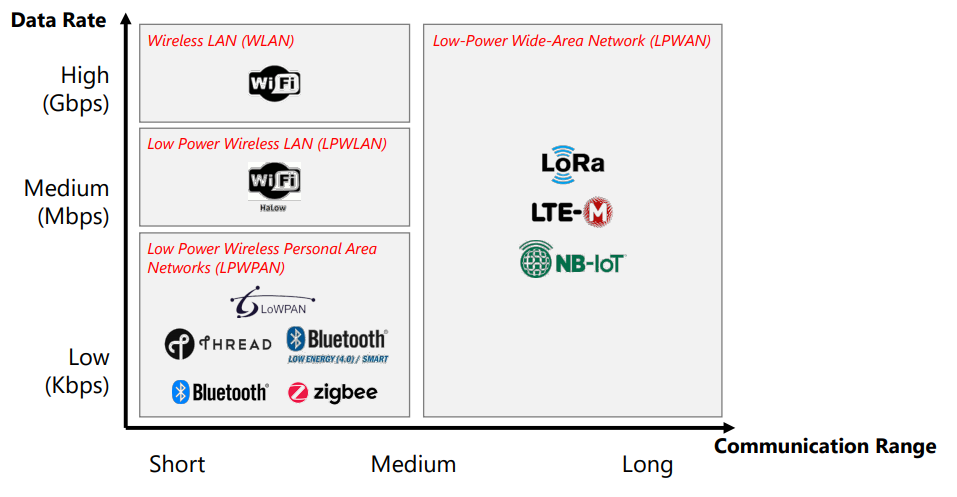
\includegraphics[scale=0.6]{assets/iot_protocols.png}
    \caption{Different IoT Protocols for Different Environments.}
\end{figure}
\begin{figure}[!htb]
    \centering
    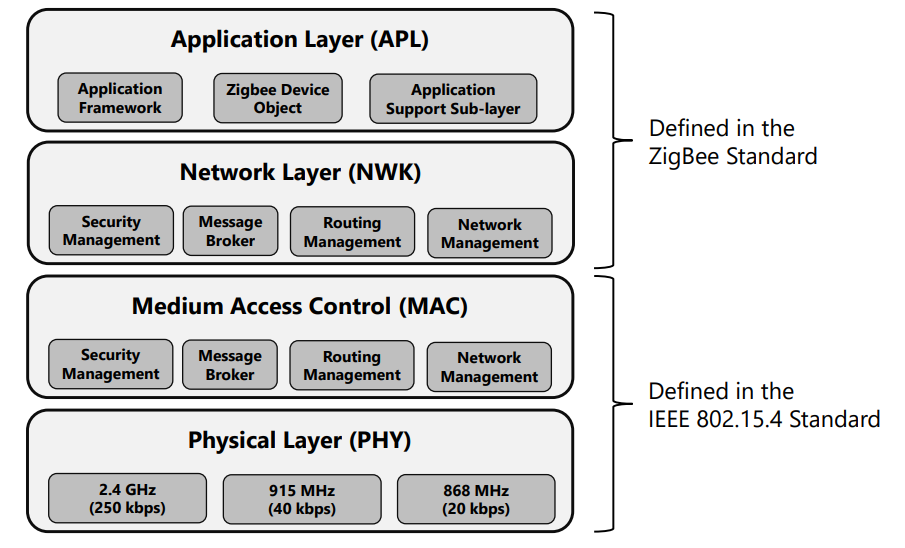
\includegraphics[scale=0.6]{assets/zigbee.png}
    \caption{Zigbee Protocol Stack.}
\end{figure}
\begin{figure}[!htb]
    \centering
    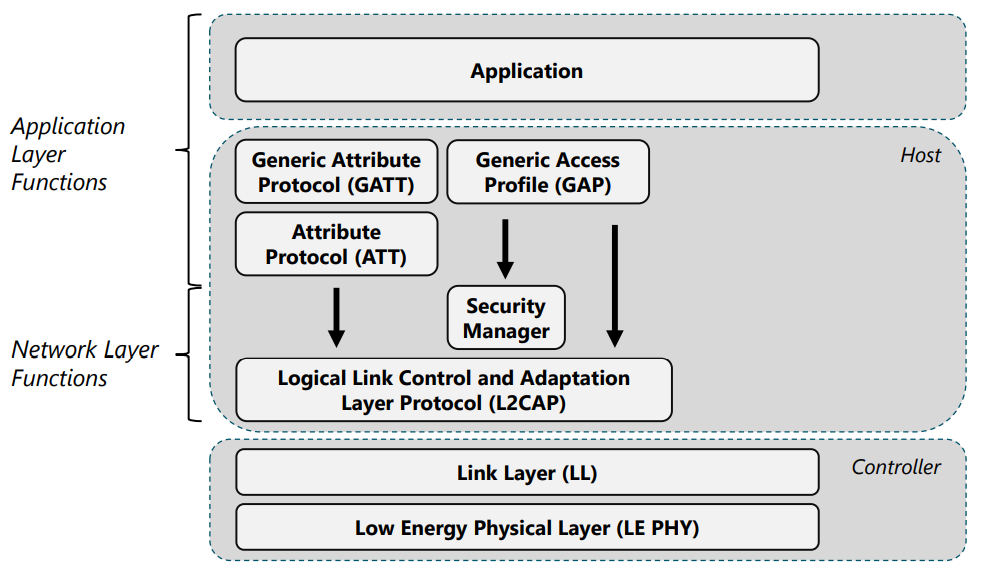
\includegraphics[scale=0.6]{assets/bluetooth_low_energy.png}
    \caption{Bluetooth Low Energy Protocol Stack.}
\end{figure}
\textbf{Intra-domain vs. Inter-domain}\newline
Internet routing works on two levels:
\itemnum
    \ii Each AS runs an intra-domain routing protocol internally
    \itemnum
        \ii Establishes routes to internal prefixes and between routers
        \ii Example protocols: OSPF, IS-IS
        \ii Run “Interior Gateway Protocol” (IGP) within ISPs
    \itemend
    \ii Each AS runs an inter-domain routing protocol on links to neighboring ASes
    \itemnum
        \ii Establishes routes to external destinations
        \ii Border Gateway Protocol (BGP)
        \ii Use “Border Gateway Protocol” (BGP) to connect ISPs. To reduce costs, peer at exchange points (AMS-IX, MAE-EAST)
    \itemend
\itemend
\begin{figure}[!htb]
    \centering
    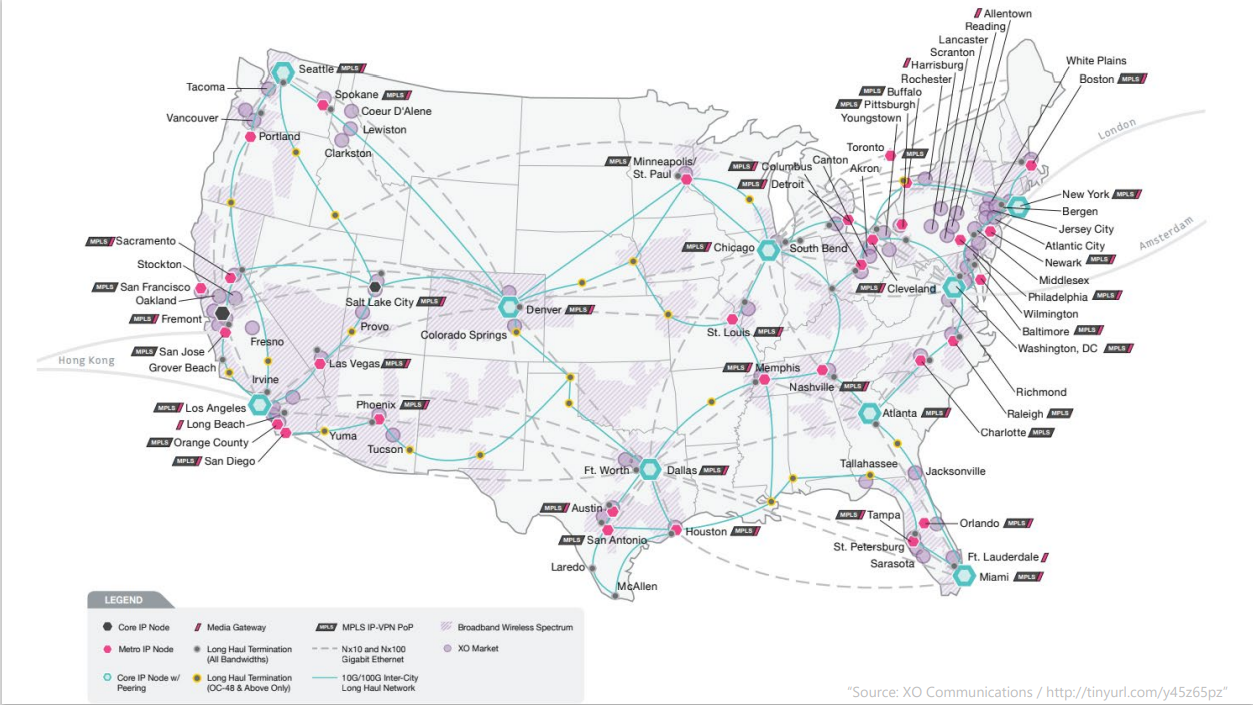
\includegraphics[scale=0.5]{assets/xo.png}
    \caption{XO Communications Backbone.}
\end{figure}
\begin{example}[XO Communications Backbone]
The dots are locations where XO Communications provides service to its users. And the lines are links. So what you do as ISP is you look at your market and you figure out where to place routers. The locations where you put routers are known as points of presence. Typically, different ISPs contract with third parties which already own fiber. A lot of these companies that already own fiber are train companies because train companies happen to already own these long secs of land that crisscross the United States. So train companies have gotten into the business of creating optical fiber deployments and they resell to ISPs.
\end{example}
\textbf{Layer 2 vs Layer 3 forwarding}\newline
L3 Routing Proactively Builds State: Control Messages, Routing \newline
L2 Switching Relies on Broadcast\newline
\textbf{Network Virtualiztion}
\itemnum    
    \ii Divide up hosts into logical groups called VLANs
    \itemnum
        \ii Like virtual machines, but for LANs (creates “virtual networks”)
        \ii VLANs isolate traffic at layer 2
    \itemend
    \ii Each VLAN corresponds to IP subnet, single broadcast domain
    \ii Ethernet packet headers have VLAN tag
    \ii Bridges forward packet only on subnets on corresponding VLAN
\itemend
There's a lot of virtualization technologies and networks which are similar to this like VRFs, VXLAN and so on. They all kind of work in the same way, they all kind of take the networks and divide them up into pieces. When you build networks, VLANs are really important to use. Virtual networks are very important because they segment your network up and they can keep your private data away from your public data. So they're very important security primitive.\newline
\textbf{Delivery Methods}
\itemnum
    \ii Unicast
    \itemnum
        \ii One source, one destination
        \ii Widely used (web, cloud, streaming; many protocols)
    \itemend
    \ii Broadcast
    \itemnum
        \ii One source, all destinations
        \ii Used to disseminate control information, perform service discovery
    \itemend
    \ii Multicast
    \itemnum
        \ii One source, several (prespecified) destinations
        \ii Used within some ISP infrastructures for content delivery, overlay networks        
    \itemend
    \ii Anycast
    \itemnum
        \ii One source, route to “best” destination
        \ii Used in DNS, content distribution, service selection
    \itemend
\itemend
\textbf{Multicast Approaches}\newline
Source-Specific Trees\newline
\itemnum
    \ii Each source is the root of its own tree
    \ii One tree per source
    \ii Tree consitst of shortest paths to each receiver
\itemend
Shared Tree
\itemnum
    \ii One tree used by all members of a group
    \ii Rooted at “rendezvous point” (RP)
    \ii Less state to maintain, but hard to pick a tree that’s “good” for everybody
    \ii Ideally, find a “Steiner tree” minimum-weighted tree connecting only the multicast member(NP-hard)
    \ii Instead, use heuristics(E.g., find a minimum spanning tree)
\itemend
\newpage
\section{Week 2 Lecture: Devices: IoT circuits}
\section{Appendix}
\renewcommand{\listtheoremname}{List of Definitions and Theorems}
\listoftheorems[ignoreall,show={theorem,definition}]

\listoftodos

\end{document}